\myparagraph{Préparation et pré-traitement}
\vspace{\baselineskip}
\\
\noindent L'évaluation de la segmentation avec des vidéos va s'effectuer non pas avec la caméra, mais avec un matériel vidéo virtuel. En effet, il n'est pas réaliste de pouvoir travailler sur le terrain. La commande "segnet-camera" permet de fournir en option le matériel qui doit être utilisé, par exemple "/dev/video0" pour la caméra. Le module "v4l2loopback"\footnote{\url{https://github.com/umlaeute/v4l2loopback}} permet de créer un matériel vidéo virtuel "/dev/video1". Ce matériel permet de recevoir un flux vidéo, qui pourra alors alimenter l'utilitaire "segnet-camera", comme le ferait la caméra. Le flux vidéo est produit par l'utilitaire "gstreamer" avec comme données d'entrées le fichier de la vidéo et dirigé vers le matériel vidéo virtuel "/dev/video1".
\vspace{\baselineskip}
\\
\noindent La difficulté réside dans le fait que le matériel vidéo virtuel et le flux vidéo doivent être compatibles avec ce que l'utilitaire "segnet-camera" s'attend, et qui a été conçu pour être compatible avec une caméra. 
\vspace{\baselineskip}
\\
\noindent Le diagramme de la figure \ref{fig:arch_segmentation_video} résume à haut niveau les relations entre ces éléments. Pour comparaison, le diagramme de la figure \ref{fig:arch_segmentation_camera} montre la segmentation avec la caméra. 
\begin{figure}[H]
    \centering
    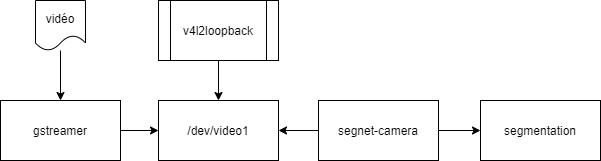
\includegraphics[width=.65\textwidth]{arch_segmentation_video}
    \caption[Diagramme d'architecture de la segmentation d'une vidéo]{Diagramme d'architecture de la segmentation d'une vidéo}
    \label{fig:arch_segmentation_video}
\end{figure}
\begin{figure}[H]
    \centering
    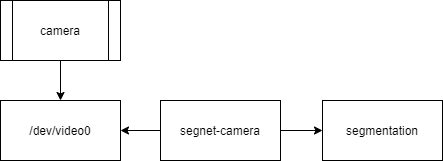
\includegraphics[width=.5\textwidth]{arch_segmentation_camera}
    \caption[Diagramme d'architecture de la segmentation avec la caméra]{Diagramme d'architecture de la segmentation avec la caméra}
    \label{fig:arch_segmentation_camera}
\end{figure}
\myparagraph{Segmentation et évaluation}
\vspace{\baselineskip}
\\
\noindent Les tests de performance de la segmentation de vidéos se déroulent de la manière précisée dans la section "\ref{section:strategie_test_inference} \nameref{section:strategie_test_inference}". 
\vspace{\baselineskip}
\\
\noindent L'un des avantages de l'utilitaire "gstreamer" est de pouvoir contrôler la résolution et le nombre d'images par seconde (\acrshort{fps}) de la vidéo qui doit être segmentée. Les différentes résolutions et \acrshort{fps} qui désirent être exécutées sont préparées dans un script "shell" écrit pour l'occasion. Le script s'occupe de démarrer gstreamer avec les bons paramètres, et en parallèle de démarrer la segmentation avec "segnet-camera". Un jeu de résolution peut être testé unitairement\footnote{\url{https://github.com/vince7lf/gae724/blob/master/run_deepscene.sh}}, ou plusieurs en séquence\footnote{\url{https://github.com/vince7lf/gae724/blob/master/run_deepscene_batch.sh}}. 
\vspace{\baselineskip}
\\
\noindent Les résolutions et images par seconde qui ont été testées sont résumées dans le tableau \ref{table:resolutions_to_be_tested}. 
\vspace{\baselineskip}
\\
\noindent Deux vidéos ont été utilisées pour tester la segmentation. La première vidéo est utilisée pour tester l'inférence avec une vidéo du site d'étude, et qui a été fournie gracieusement par l'\acrshort{apcpontjc}. Cette première vidéo est intéressante, car elle est filmée en mouvement par un cycliste. Dans un interval de 30 secondes, l'angle de vue change rapidement. La piste cyclable est bordée d'un muret côté sud, et de la route avec les voitures qui circulent côté nord. Même si la journée est ensoleillée, la surface de la piste est aussi à un moment humide.
\vspace{\baselineskip}
\\
\noindent La seconde vidéo est utilisée pour tester la segmentation avec les différentes résolutions et images par seconde. C'est une vidéo d'une petite piste cyclable qui est dans mon quartier, et que j'ai prise en marchant avec mon téléphone intelligent. La vidéo est intéressante, car dans un interval de 30 secondes l'état de la piste passe d'une scène ensoleillée à ombragée, sèche à mi-sèche, avec un petit ou gros banc de neige en bordure, ou qui s'aventure un peu sur la piste, bordée d'herbe mouillée ou sèche.